\chapter{Entwurfsmuster}

\section{Entwurfsmuster: Erbauer}
Die nachfolgende Abbildung zeigt ein vereinfachtes UML-Diagramm der
Klasse \textit{IsaacLevelGenerator}, welches das Interface
\textit{ILevelGenerator} implementiert. Das Interface dient als
Abstraktion eines beliebigen Level-Generators, der
\textit{IsaacLevelGenerator} ist eine konkrete Implementation.

Es handelt sich hierbei um das Entwurfsmuster \textbf{Erbauer}.
In diesem Fall ist \textit{IsaacLevelGenerator} ein konkreter Erbauer. 
Durch die Verwendung des \textit{ILevelGenerator} Interfaces kann
die Konstruktionsmechanik für ein Level jedoch beliebig ausgetauscht
werden.

Die \textit{next()}-Funktion des \textit{IsaacLevelGenerator}
beschreibt eine mehrschrittige komplexe Logik zur Erzeugung von
\textit{Level}-Objekten. Sie kann genutzt werden, um immer wieder
gleiche Objekte zu generieren. Die Verwendung eines \textit{Erbauers}
erlaubt die Trennung zwischen der komplexen Erstellung eines Objektes
und  seiner Klassenrepräsentation. Zudem versteckt der Generator die
interne Repräsentation während der Level-Erstellung. Letztlich wird
nur das fertige Produkt zur Verfügung gestellt.

Die Verwendung des \textit{Erbauer}-Musters erhöht die Modularität
durch Austauschbarkeit und die Verwendung eines Interfaces. Zudem
vermindert es die Komplexität, da unterschiedliche komplexe
Erzeugungsprozesse jeweilig in einem \textit{Erbauer} gebunden sind.
Alles zusammen erlaubt auch einfache Erweiterbarkeit, da immer neue
\textit{Erbauer} anstelle des Interfaces gesetzt werden können.

\vspace{0.5cm}
\begin{figure}[H]
    \centering
    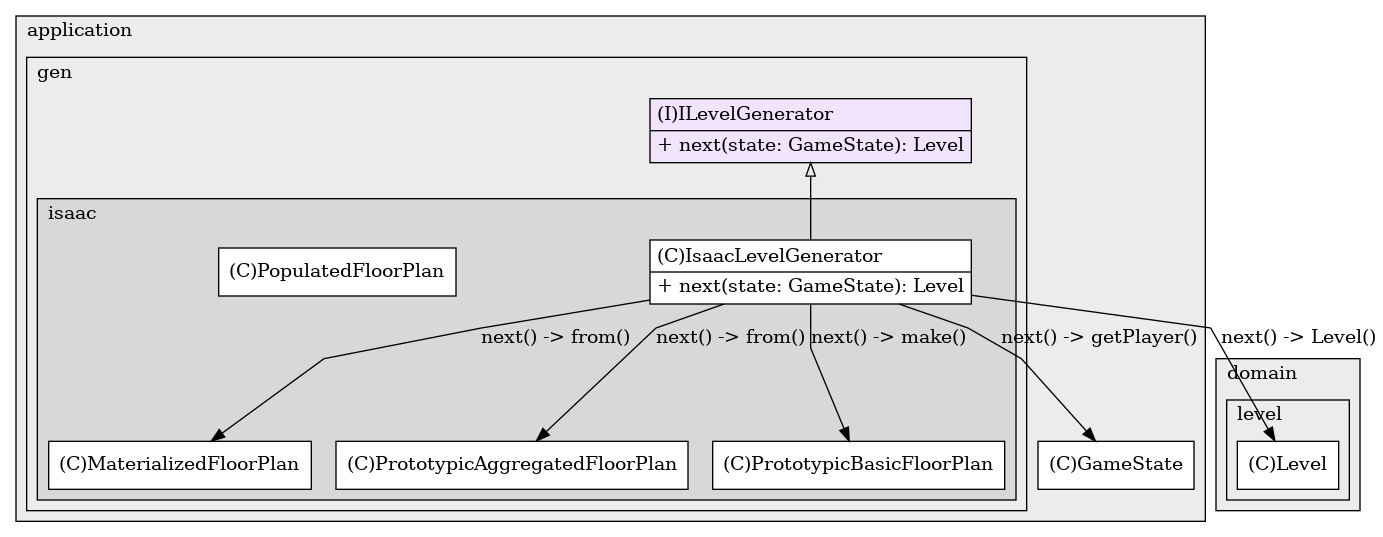
\includegraphics[width=1\linewidth]{Bilder/Visualisierung/IsaacLevelGenerator_structure.png}
    \caption{Entwurfsmuster: Erbauer}
\end{figure}

\section{Entwurfsmuster: Kompositum}
Die nachfolgende Abbildung zeigt das UML-Diagramm der Klassen
\textit{Buffer} und \textit{CompositeBuffer}, wobei letztere von
ersterer erbt. Beide Klassen finden Verwendung in der Spielanzeige
auf der Konsole. Dabei werden statische \textit{Sprites} mithilfe
der Klasse \textit{Buffer} beschrieben, komplexere Anzeigen, bei denen
dynamische Änderungen auftreten können mithilfe der Klasse
\textit{CompositeBuffer}.

Es handelt sich hierbei um das Entwurfsmuster \textbf{Kompositum}. 
Objekte der beiden Klassen lassen sich gemeinsam zu einer Baum-Struktur
zusammensetzen. Beide Typen sind gleichwertige Komponenten. Die
\textit{Buffer} sind dabei Blätter bzw. einfache Elemente, wohingegen
\textit{CompositeBuffer} wie Container funktionieren und die Kinder
verwalten. 

In der Gesamtheit verhalten sie sich wie eine Einheit. Sie teilen sich
alle Funktionen der zugrundeliegenden Klasse \textit{Buffer}. So etwa
die Funktion \textit{toString()}, welche den Buffer-Inhalt in einen
String für die Konsole überführt oder die Funktion \textit{render()},
welche rekursiv den Baum vom Wurzel-Element ausgehend traversiert und
entsprechende Updates veranlasst.

In der Abbildung ist zu sehen, dass die Klasse
\textit{CompositeBuffer} genutzt wird, um Anzeigen (\textit{Views})
zu erstellen. Die bedeutenste Klasse ist dabei
\textit{TerminalInterface}, da sie die Hauptanzeige modelliert.
Die Klasse \textit{CompositeBuffer} bietet jedoch, im Gegensatz zum
\textit{Buffer}, zur Einfachheit und Effizienz die Möglichkeit
zwischen fixierten \textit{fixed()} und dynamischen \textit{dynamic()}
Elementen zu unterscheiden.

\vspace{0.5cm}
\begin{figure}[H]
    \centering
    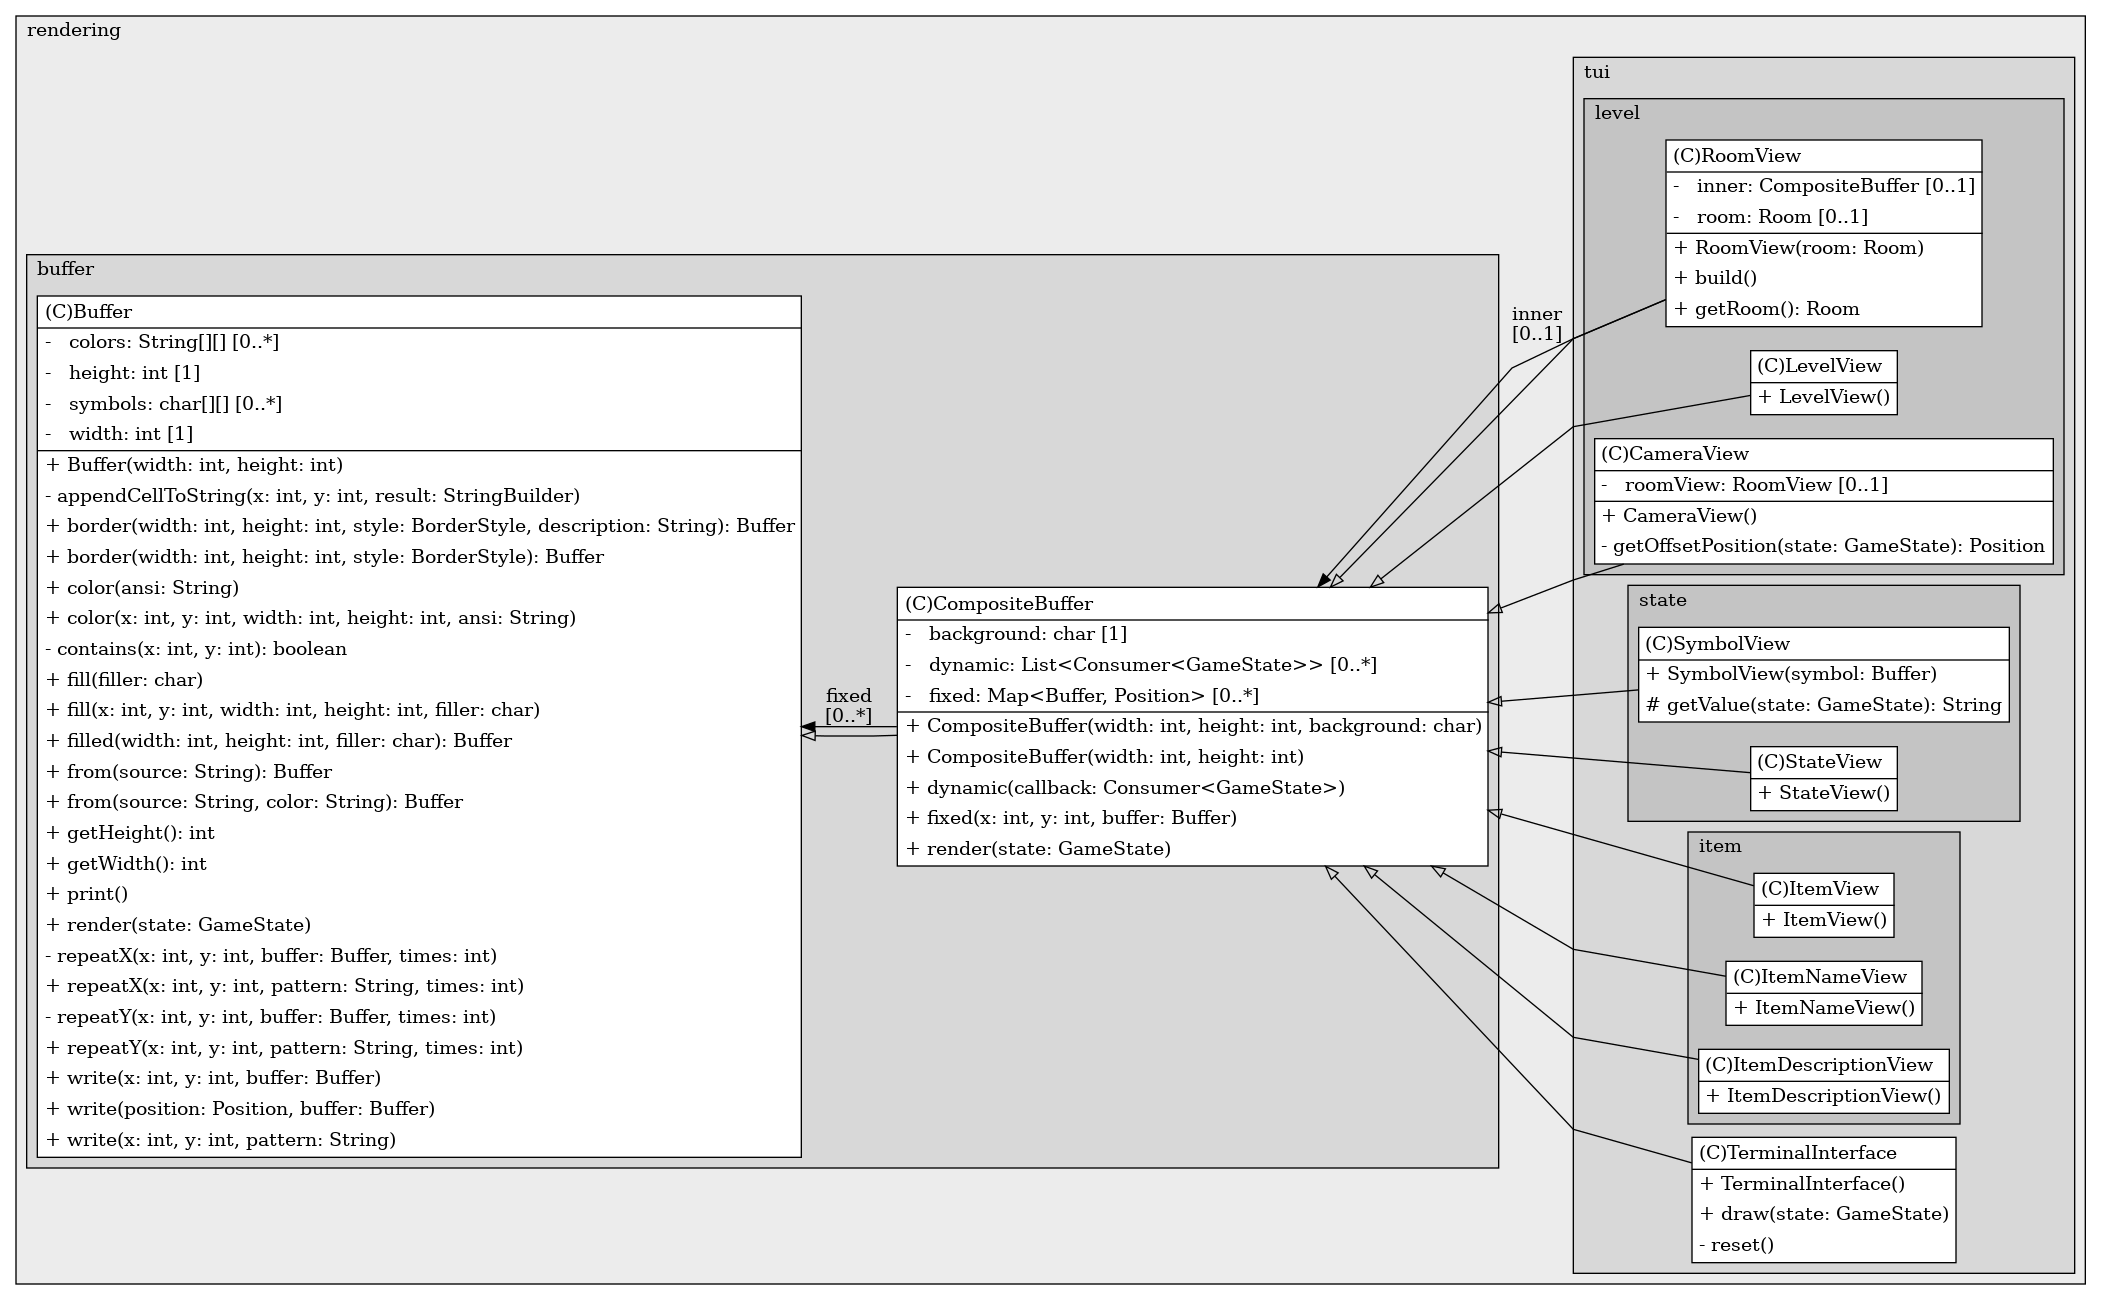
\includegraphics[width=1\linewidth]{Bilder/Visualisierung/CompositeBuffer_structure.png}
    \caption{Entwurfsmuster: Kompositum}
\end{figure}